\documentclass{article} 
\usepackage[left=0.75in,top=0.6in,right=0.75in,bottom=0.6in]{geometry} % Document margins
\usepackage{tabularx}
\usepackage{fancyvrb}
%\usepackage[hidelinks]{hyperref}
\usepackage{graphicx}
\usepackage{float}
\usepackage{fancyhdr}
\usepackage{geometry}
\usepackage{lastpage}
\usepackage{tabu}
\usepackage{hyperref}

\geometry{
  top=1in,            % <-- you want to adjust this
  inner=0.5in,
  outer=0.5in,
  bottom=1in,
  headheight=5ex,       % <-- and this
  headsep=4ex,          % <-- and this
}

\pagestyle{fancy}
\fancyhf{}
\rhead{\Large\textit{Old Dominion University}}
\lhead{\Large\textit{ECE 432: Assignment 7}}
\cfoot{Page \thepage \hspace{1pt} of \pageref{LastPage}}
\renewcommand{\footrulewidth}{1pt}

\begin{document}

%----------------------------------------------------------------------------------------
%		 TITLE PAGE
%----------------------------------------------------------------------------------------

\begin{titlepage}

\vspace*{45 pt}
\begin{center}
\Huge{\bf CS 432/532:  Web Science}\\
\huge{Spring 2017\\}

\vspace{60 pt}
\Huge\underline {Assignment 7}\\

\vspace{10 pt}
\Huge{Michael Micros}\\\

{\Large \bf {Instructor: Michael L. Nelson}}\\

\vspace{230 pt}
{\huge \bf {Old Dominon University}}\\
{\huge \bf {Norfolk, Virginia}}\\

\vspace{10 pt}
\today

\end{center}
\end{titlepage}




%----------------------------------------------------------------------------------------
%		PROBLEM 1
%----------------------------------------------------------------------------------------

\section*{{\underline{\huge {Problem 1:}}  Finding the ``substitute you"}}
It is important to note that for all the questions of this assignment  sample code from the ``Collective Intelligence Programming" book was used. Therefore all functions for calculating correlations, providing recommendations and loading in data from MovieLens dataset.

In order to find a user that will represent my taste in movies, it was first necessary to filter the users and isolate the users that were most simillar to me. After reading through all the users in the ``u.users'' file, I created a list of all users that were 24 years old, had 'student' as occupation, and were male.


\begin{figure}[H]
 \centering
 	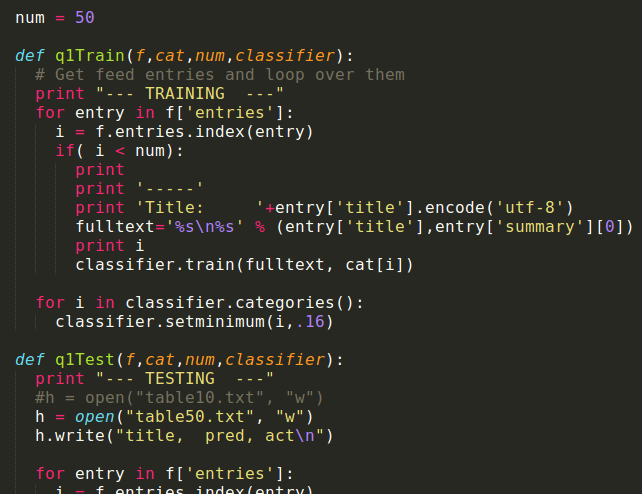
\includegraphics[height=6 cm]{p1.png}
  \caption{Code for filtering users by age,gender and occupation}
\end{figure}

 For 3 users from the list I displayed their highest rated and lowest rated films and selected the user with whom I identified the most. The results for the 3 users are writen in a text file named ``Alter Egos''. The user I selected as the ``substitute me" in the list was User 73. Though his top picks were not my favorite films, User 73 seemed to have the best taste out of all the other users.


\begin{figure}[H]
 \centering
 	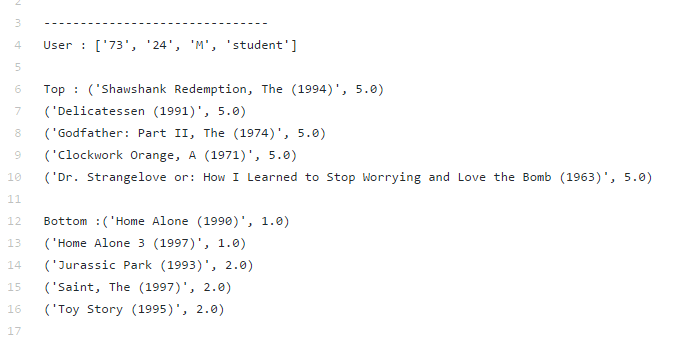
\includegraphics[height=8 cm]{alter.png}
  \caption{User 73's highest and lowest rated films.}
\end{figure}


%----------------------------------------------------------------------------------------
%		PROBLEM 2
%----------------------------------------------------------------------------------------

\section*{{\underline{\huge {Problem 2:}}  Most and Least correlated Users to ``me"}}

In order to find the 5 most and least correlated users to the ``substitute me" I used the topMathes() function provided in the ``Collective Intelligence" book. This functions computes the Pearson correlation between a desired User and all the users in the database. The only problem with this function is that it computes the correlation based on common rated movies without taking into account how many films both users have seen and rated. This means that if 2 users have only one common rated film and gave it the same score they will have a perfect correlation. That obviously means are results will be quite unreliable. To avoid this problem I modified the code in the sim\_pearson() function to compute the correlation for users that had more than 20 rated movies in common. The results were stored in the file ``Recommended Users" file. 


\begin{figure}[H]
 \centering
 	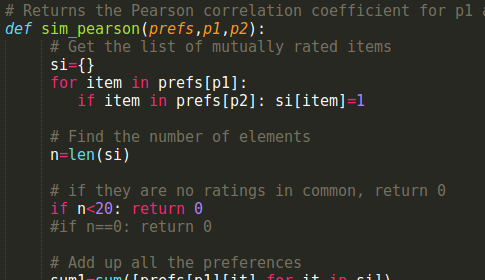
\includegraphics[height=6 cm]{sim_p.png}
  \caption{Modification in sim\_pearson() function. Compute correlation between user that have more than 20 films in common.}
\end{figure}


\begin{figure}[H]
 \centering
 	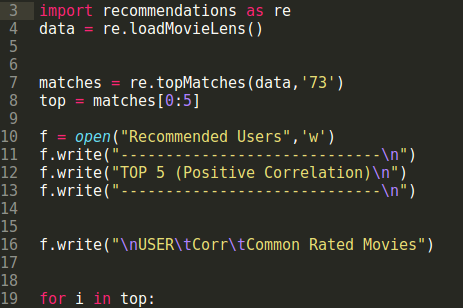
\includegraphics[height=7 cm]{p2.png}
  \caption{Code from part2.py}
\end{figure}

\begin{figure}[H]
 \centering
 	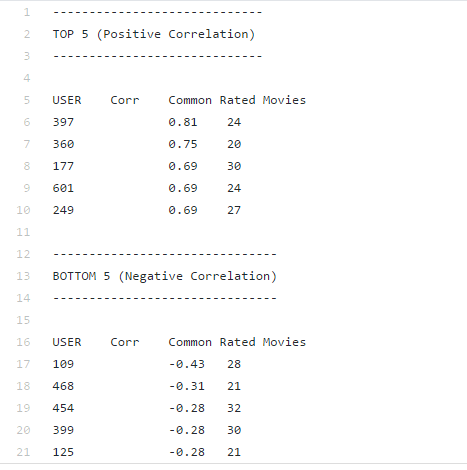
\includegraphics[height=10 cm]{p2results.png}
  \caption{Top 5 and Bottom 5 correlated Users}
\end{figure}

\vspace{20 pt}
%----------------------------------------------------------------------------------------
%		PROBLEM 3
%----------------------------------------------------------------------------------------

\section*{{\underline{\huge {Problem 3:}} Top 5 and Bottom 5 recommendations}}
In order to generate ratings for the films I have not yet seen, the getRecommendations() function was used for User 73 (my alter ego). This function goes through all the users that I am positively correlated to and finds which films they have rated that I have not seen. Greater weight is given to users that are more correlated to me. Finally, an average of all the scored is computed, which is the predicted rating for the unseen film.

I believe this method could be modified to include also the users that I was negatively correlated to. If someone I have completely opposite taste with rates a movie terribly, I might enjoy it. The way the getRecommendation() function currently works does not account for such cases.

The results for the top and bottom 5 recommendations are saved in the ``Best \& Worst Recommendations'' file.

\begin{figure}[H]
 \centering
 	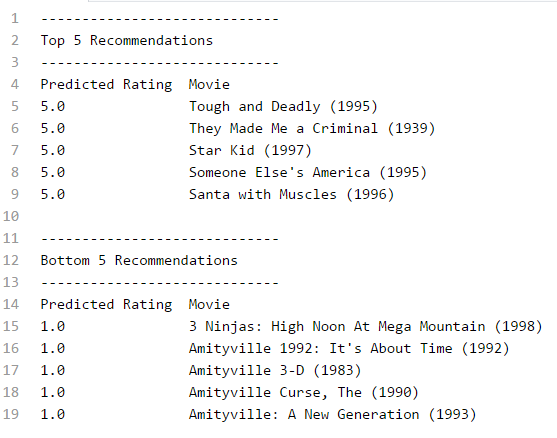
\includegraphics[height=10cm]{rec.png}
  \caption{Top 5 and Bottom 5 correlated Users}
\end{figure}

\begin{figure}[H]
 \centering
 	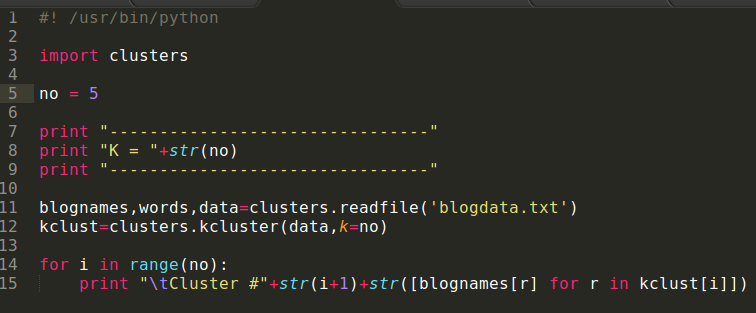
\includegraphics[height=10 cm]{p3.png}
  \caption{The code for part3 (part3.py)}
\end{figure}

\newpage



%----------------------------------------------------------------------------------------
%		PROBLEM 4
%----------------------------------------------------------------------------------------

\section*{{\underline{\huge {Problem 4:}} Correlations to my favorite and least favorite films}}
In order to find correlations to my favorite and least favorite films it was necessary to slightly modify the loadMovieLens() function. In all the previous parts the u.data was stored in a dictionary with the 'user id ' as the default key. The change that needed to be made was to make the 'movie id' the default key. This is equivalent to transforming the dictionary as is mentioned in the tectbook. Then the topMatches() function is used on the 2 films in order to generate the most correlated films. Before, when calling this function we were comparing 2 users and looking at which movies they have rated. Now we are comparing 2 movies and looking at which users have rated them.

The film chosen as my favorite film was 'Reservoir Dogs' with a movie id of '156'. My least favorite was 'Phat Beach' with a movie id of '1162'.

\begin{figure}[H]
 \centering
 	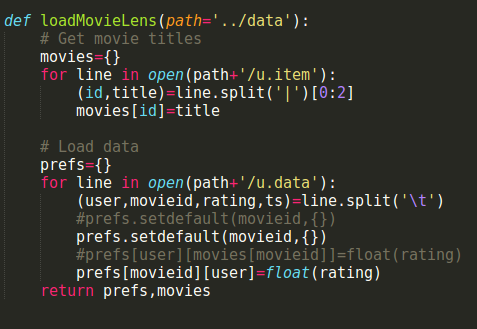
\includegraphics[height=8cm]{load.png}
  \caption{Modified loadMovieLens() function}
\end{figure}

\begin{figure}[H]
 \centering
 	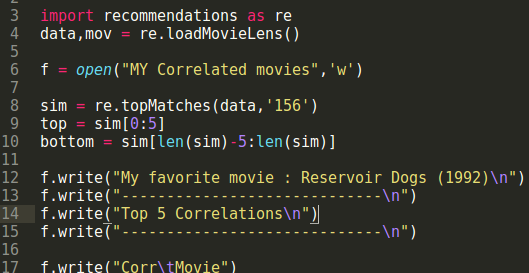
\includegraphics[height=7cm]{part4.png}
  \caption{Code for part4 (part4.py)}
\end{figure}

\newpage

The results for the 5 most correlated films to Reservoir Dogs were not films that I really knew, but the results were not accurate. I have not seen any of them and after researching them I was only really convinced that 3 were worth watchng. 'Murder, My Sweet (1944)' and 'Thieves (Voleurs, Les) (1996)' seemed like they would be interesting films. But I really want to see 'No Escape (1994)' because the thought of Ray Liotta as an action hero is just hilarious to me. As for the 5 worst correlations I have no objections since all of them are 90's rom coms. It is interesting to note that almost all of the suggestions are in the same decade as 'Reservoir Dogs' meaning that the users(most influencial) were probably all of a certain generation that had watched all these films throughout the 90s.

\begin{figure}[H]
 \centering
 	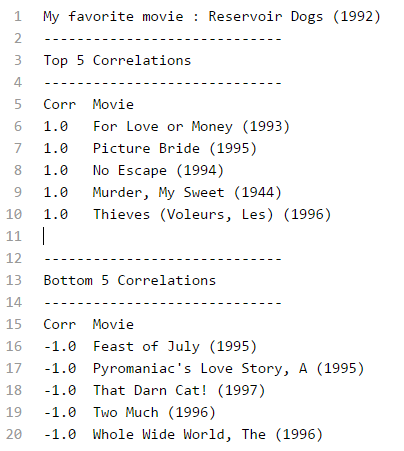
\includegraphics[height=10cm]{tcorr.png}
  \caption{Top 5 and Bottom 5 correlations for 'Reservoir Dogs'}
\end{figure}

The results for the 5 most correlated films to 'Phat Beach' seemed correct in the sense that they were similar to the target film, with the exception of 'A time to kill' and '7 years in Tibet'. The 5 worst corellated films also seemed very accurate with the 'Usual Suspects' standing out as a pretty good movie , and was expecting as a positive correlation for 'Reservoir Dogs'(``Gimme the keys you c*******er!! -- I love that scene). These correlations follow a similar pattern to the one noticed previously, in that the majority of them are 90s films.

\begin{figure}[H]
 \centering
 	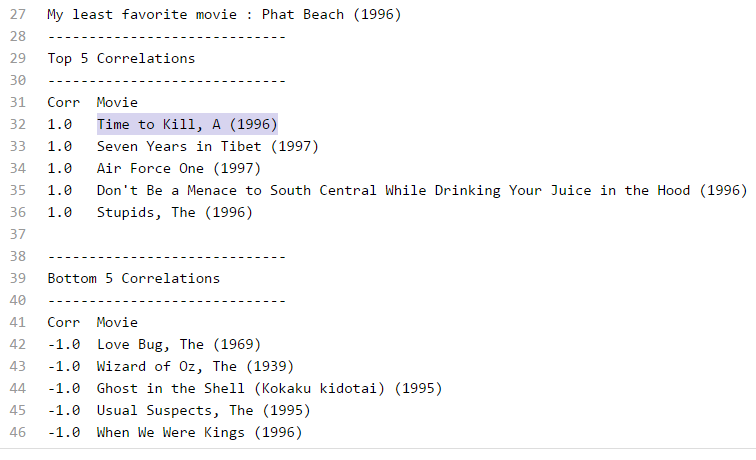
\includegraphics[height=10cm]{corr2.png}
  \caption{Top 5 and Bottom 5 correlations for 'Phat Beach'}
\end{figure}



%----------------------------------------------------------------------------------------
\end{document}
